
\subsection{Introduction}
The goal of this report is to describe the procedure performed by the group 3 for the phase 1 and 2 of the GIS-Project in the Winter Semester 2012/13.
The main task for phase 1 regards the search for further data and its integration on the data-model using an automatic or semi-automatic process. The operations involved a large number of data exchanging through different formats and a large number of  applications, such as SQL, ArcGis, FME and Excel were applied. Though, it is hard to establish an unique and solid procedure which could be systematically repeated.
After the integration of the required data, the indicators Apartments/Volume (m3) and Number of Residents/Apartment were calculated and, in the case of the first indicator, different values were obtained since they were grouped by the attribute Age of the Building.
The phase 2 comprises the actual estimation of the residential annual electricity consumption on the area of interest. Therefore, all integrated data from phase 1 is gathered in an appropriate algorithm, which relates households and annual electricity consumption.
The final result for the households average is 1.584, in contrast to the statistical one: 1.65 (Amt für Statistik Berlin-Brandenburg, 2011). That led for an average annual electricity consumption range of 2671 - 2931 kWh per apartment.
A further research towards a complete automation of the process is recommended and normally requires programmed scripts (e.g in Java) which might deal direct with both the stored data and the data to be integrated from other sources (e.g WMS and WFS), and also perform the final algorithm.
\subsection{Data Sources}
There are many sources of data available which can be integrated either directly by a simple spatial relationship or by joining operations which might become complex depending on the structure differences.\\ 
In the case of Berlin, the FIS-Broker database (http://fbinter.stadt-berlin.de) presents a large and spatially located amount of statiscal and survey data regarding social, economical and infra-structural fields. It is the most important source used during the accomplishment of the tasks.
The figure 1 elucidates the whole process divided into three steps – searching, processing and integrating:\\
\begin{figure}[ht]
	\centering
	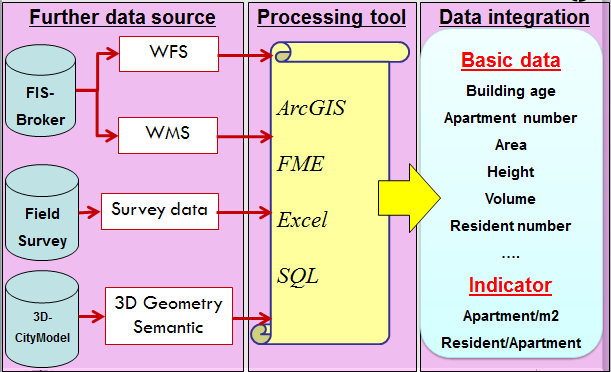
\includegraphics[width=0.9\textwidth]{phase1/group3/fig1.png}
	\caption{Data Workflow}
	\label{fig:figure1}
\end{figure}
As figure \ref{fig:figure1} shows, the sources of data consist basically on the FIS-Broker, the 3D City-Model, which provides all geometric and semantic required information, and the so called "Field Survey", consisting of a survey previously realized in the Moabit area that gathered information for random buildings regarding its number of apartments. \\
Depending on the application, many other sources can be integrated, enabling such a variety of possible calculations. The exact type of data depends also on the method to be used. The more detailed the algorithm, the more data is required. 
\subsection{Data Acquisition }
\subsubsection{WMS}

The WMS provides the web map services as a raster map. Normally, only the color information and legend are provided, but not the exact data. However, it is still an important data source and there are plenty of map services provided by WMS. In FIS-Broker database, most of data such as the building age group, proportion of different age group can be accessed by using WMS. 
In this project, a whole process of getting WMS data in FIS-Broker was created: \\
1. Get the link to URLfor WMS service from:\\
www.stadtentwicklung.berlin.de\\
2. Using ArcGIS connect to the WMS.\\
3. Set the coordinates system\\
4. Export map by choosing .tiff format in high resolution (300 dpi) and geotiff Tags\\
5. Combine the export map (Spatial Analyst Tools->Local->Combine)\\
6. Re-color raster data and make new legend\\
7. Zonal statistics as table\\
8. Join statistics table and new legend to the feature layer\\

The WMS information is saved in the feature layer after all these steps above. But maybe there are some errors in the boundary due to the data resolution. \\
\begin{figure}[ht]
	\centering
	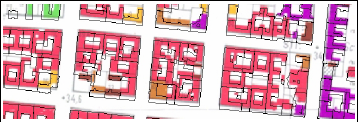
\includegraphics[width=0.9\textwidth]{phase1/group3/fig2.png}
	\caption{Mismatch of Overlap (Carrion, 2010)}
	\label{fig:figure2}
\end{figure}
\subsubsection{WFS}

The WFS  is the short term for Web Feature Service in which the graphical features can be requested from the services. Both geometry and semantic data are provided by WFS. Therefore, not the color information, but the database can be easily requested by the users compare to WMS. For example, in WMS, the information of building age is given in a time period which is shown in the legend, while in WFS it is provided the exact construction year, as a vector data, which is more specific and useful. \\
To get WFS data, several steps are needed  as follows:\\

1. Applying FME Intergration Console - add FME extension to ArcGIS

2. Add FME connection

3. Select WFS data Format

4. Set parameter.\\

Some feature data like building and statistical block as well as semantic data like number of residents in each block are extracted from WFS. However, the WFS services are not commonly open. The FIS-Broker WFS services is not availabe anymore available, due to security reasons.

\subsubsection{Field Survey}
The energy consumption have a tightly relationship with number of apartments. Therefore a field survey for apartment number is necessary. This survey is done based on different building age group. For each building group, at least 10 buildings were selected to count the number of apartment by counting the ring bells.
\subsubsection{CityGML}
Also some useful data can be obtain from CityGML, especially 3D geometry data, such as the footprint area and building height. Because only the residential volume is important in this project, the height of the building is calculate by removing the roof height.
\subsection{Integration}
The aim of Phase I is to get two important indicators: Apartment/Volume(m3) and Resident/Apartment. To calculate these two indicators, not only the data from different data sources is required, but also different tools (FME, ArcGIS, SQL, Excel) should be integrated together.
\subsubsection{Age of Buildings}

The attribute age of buildings specifies the exact year of construction for the buildings. For cities like Berlin which have a long history, the building age may vary from more than 100 years to recent 1 or 2 years. As architectural properties might not vary so deeply during years or even decades, this attribute is better represented by a range of values. \\

Therefore, the attribute age class was separated into 6 groups: 1889-1918, 1919-1945, 1946-1961, 1962-1974, 1975-1993 and 1994-2012.\\
\subsubsection{Apartment Number / Volume}
The number of apartment is the key value for the next steps. As it is impossible to do the survey for all buildings in the test area, this indicator was introduced. It is calculated from the field survey data and then can be easily gotten the apartment number of other buildings by multiplying this indicator with the building volume.

As a further data to be attached on the calculations, a survey was performed on the area of interest, with the goal of obtaining the number of apartments on the region. Thus, the survey data provides the counting of the ring bells for a selected group of buildings.

The process to join all the information must contain an export of the surveying data on the database. Then, the GMLID have to be joined accordingly – this is realized by the address of the buildings, as both the surveying data and the data model provide it. 

The following script is an example of a join by the address. It shows basically the final step, once the surveying data is already imported on the data model:
\begin{lstlisting}
select  street, house_number, apartment, a.id,
b.building_id,co.gmlid
from join_surveying js
inner join address a
on js.strasse=a.street and js.hnr=a.house_number join
address_to_building b
on a.id=b.address_id join cityobject co
on b.building_id=co.id;
\end{lstlisting}

As the footprints are  to provide the area of the buildings, one must aggregate the height information. A close look on the database highlights the existence of three different heights per building:
\begin{itemize}
\item Measured\_Height (Hm): representing the total height of the building
\item H\_Trauf (Ht): the lower height of the roof
\item H\_First (Hf): the upper height of the roof
\end{itemize}

So, the real height (Hr) is calculated through the following relationship:
\begin{align}
Hr=Hm-(Hf-Ht)
\end{align}


The real volume for each building is trivially obtained from the multiplication of the footprint area with the real height. Then, the indicator " apartment Number / Volume(m3)” is performed like:\\
\begin{align}
I = \frac {\sum\limits_{k=1}^n T_{k}}{\sum\limits_{k=1}^n V_{k}}
\end{align}


Where:\\
I = Indicator (Apartment number / Volume(m3))\\
T = number of apartments of building k\\
V= volume of building k\\
n = total surveyed buildings\\
\\
Afterwards, the above procedure is expanded. Each building age class receives a different indicator, as they present different periods of construction and, therefore, different architectural configurations which renders different results.\\

It is important to mention that the indicators inherit an expectation "behave". It is well known that older buildings used to have less apartment for the same amount of volume. Another socio-economic issue is related to the period right after the second World War. As the demand for new buildings was very high due to the destruction caused by the war, the short period after 1945 should present the highest indicators. \\

Also, the integration of the surveying data presents some mismatches from real data to the 3D Model. Some buildings have more than one address and vice-versa. Some garages are integrated on the buildings and, therefore, would be part of the volume calculation.\\

In order to avoid mismatches and to build reliable indicators, some unclear data were not taken into account. For the next survey missions, it is recommended to take a brief look on the 3D Data Model before going to the field, so that only reliable buildings could be selected.



\subsubsection{Number of Inhabitants}

A very important data for input in energy simulations is the number of inhabitants of the residential area of interest. Once the city model supports semantic information about the usage of the buildings, it is possible to split the inhabitants inside the buildings, and so, have an estimation of the households.\\
For this task, a WFS was provided containing the total amount of inhabitants per block. In order to obtain the total amount of inhabitants per building, a weighting by an approximation of the building volume was performed.

\begin{figure}[ht]
	\centering
	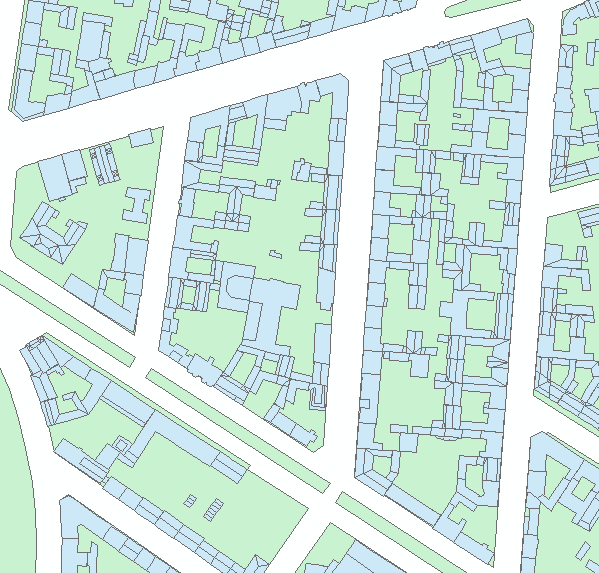
\includegraphics[width=0.8\textwidth]{phase1/group3/fig3.PNG}
	\caption{Building Footprints X Block (Self Made)}
	\label{fig:figure3}
\end{figure}

In order to calculate the number of inhabitants or residents per building, a previous selection is performed on the database, returning only the buildings which present residential purpose. As the buildings are semantically defined also by its function of usage, based on OSKA(Objektschlüsselkatalog – 2003) the following script was performed: \\

\begin{lstlisting}
select  b.id,co.gmlid, b.function, b.measured_height,
a.street, a.house_number
from cityobject co , building b, address a, 
address_to_building ab
where b.id=co.id and b.id=ab.building_id and 
ab.address_id = a.id and (
b.function='1373' or b.function='1331' or b.function='1311'
or b.function='1372' or b.function='1399' or b.function='1379'
or b.function='1381' or b.function='2199' or b.function='1301'
or b.function='1361' or b.function='1341' or b.function='1221' 
or b.function='1321' or b.function='1374' or b.function='1371'
or b.function='1231' or b.function='2131'  
or b.function='2121' or b.function='2101'   
or    b.function='2141');
\end{lstlisting}

\begin{figure}[ht]
	\centering
	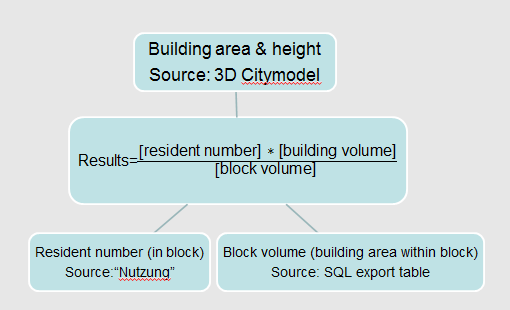
\includegraphics[width=0.8\textwidth]{phase1/group3/fig4.png}
	\caption{Inhabitants per Building (Self Made)}
	\label{fig:figure4}
\end{figure}


Figure \ref{fig:figure4} shows how to calculate the number of inhabitants in each building. In order to group the buildings per block, a spatial join is realized in ArcGis and the results are exported to the data-base. Then, as the buildings contain their “BlockId” attribute, as well as the sum of inhabitants in that block (for instance called “S” attribute), the residents shall be split into the buildings according to the next sentence:\\


$Ri= (Sk*Vi)/Vk$\\
\\
Where:\\
		Ri = Residents on building i\\
		Sk = Total number of inhabitants on block k\\
		Vi = Volume of building i\\
		Vk= Total Volume of buildings on block k

\subsection{Results}


Table 1 shows the results of Apartment/Volume for different building age group.

\begin{table}[ht]
	\centering
	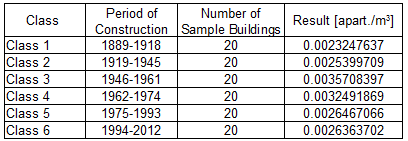
\includegraphics[width=0.8\textwidth]{phase1/group3/fig5.PNG}
	\caption{Indicator 'Apartments/Volume (m3)' (Self Made)}
	\label{fig:figure5}
\end{table}


\begin{figure}[ht]
	\centering
	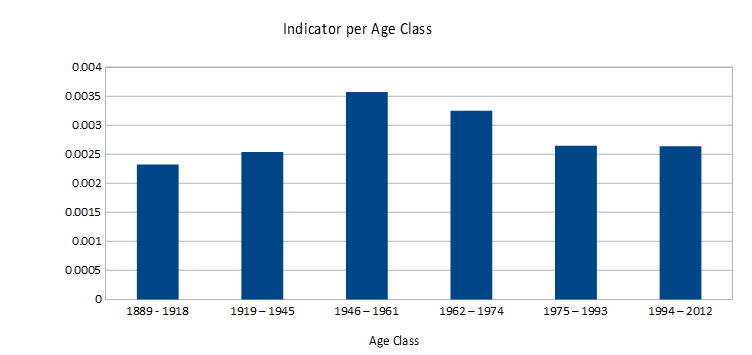
\includegraphics[width=0.8\textwidth]{phase1/group3/fig6.PNG}
	\caption{Indicators grouped by Age Class (Self Made)}
	\label{fig:figure6}
\end{figure}

Applying the indicators above, the apartment number for the whole test area can be calculated by multiplying the indicator with the building volume. Furthermore, the average household can by computed:\\
\begin{align}
Hi=\frac{Ri}{Ni}
\end{align}
Where:\\
H = Household average for building i\\
R = Total number of residents on building i\\
N = Number of apartments on building i (based on the volume)\\

The average result for the area of interest is: \textbf{H=1.584}
\\

As a validation procedure, the result might be compared to to statistical data on Figure 6. Statistically, the Mitte neighborhood presents 1.65 as household average value.

\begin{figure}[ht]
	\centering
	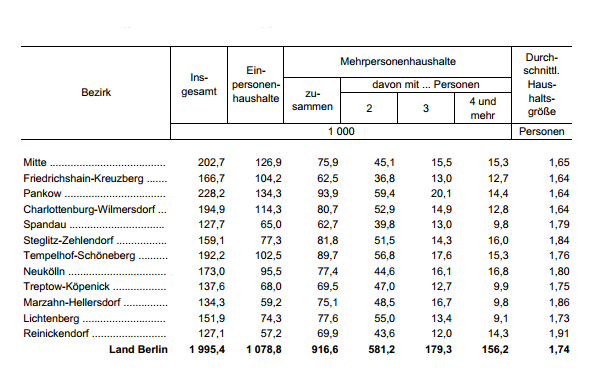
\includegraphics[width=0.8\textwidth]{phase1/group3/fig7.png}
	\caption{ Household in Berlin (Amt für Statistik Berlin-Brandenburg, 2011)}
	\label{fig:figure7}
\end{figure}